\documentclass[11pt]{standalone}
\usepackage{amssymb}
\usepackage{amsmath}
\usepackage[no-math]{fontspec}
\usepackage{unicode-math}
\usepackage{libertinus}
\usepackage{pgf,xcolor}
\usepackage{tikz}
\usetikzlibrary{arrows.meta, backgrounds}
\usepackage{pgfplots}
\usepgfplotslibrary{groupplots}
\pgfplotsset{compat=newest}

\setmainfont{Libertinus Serif}
\setmathfont{Libertinus Math}

\definecolor{my_darkgray}{HTML}{484949}
\definecolor{my_lightgray}{HTML}{F3F4F4}
\definecolor{my_darkblue}{HTML}{005A94}
\definecolor{my_lightblue}{HTML}{CCDEE9}
\definecolor{my_yellow}{HTML}{FFEC7F}
\definecolor{my_red}{HTML}{E60000}
\definecolor{my_orange}{HTML}{E87846}

\begin{document}

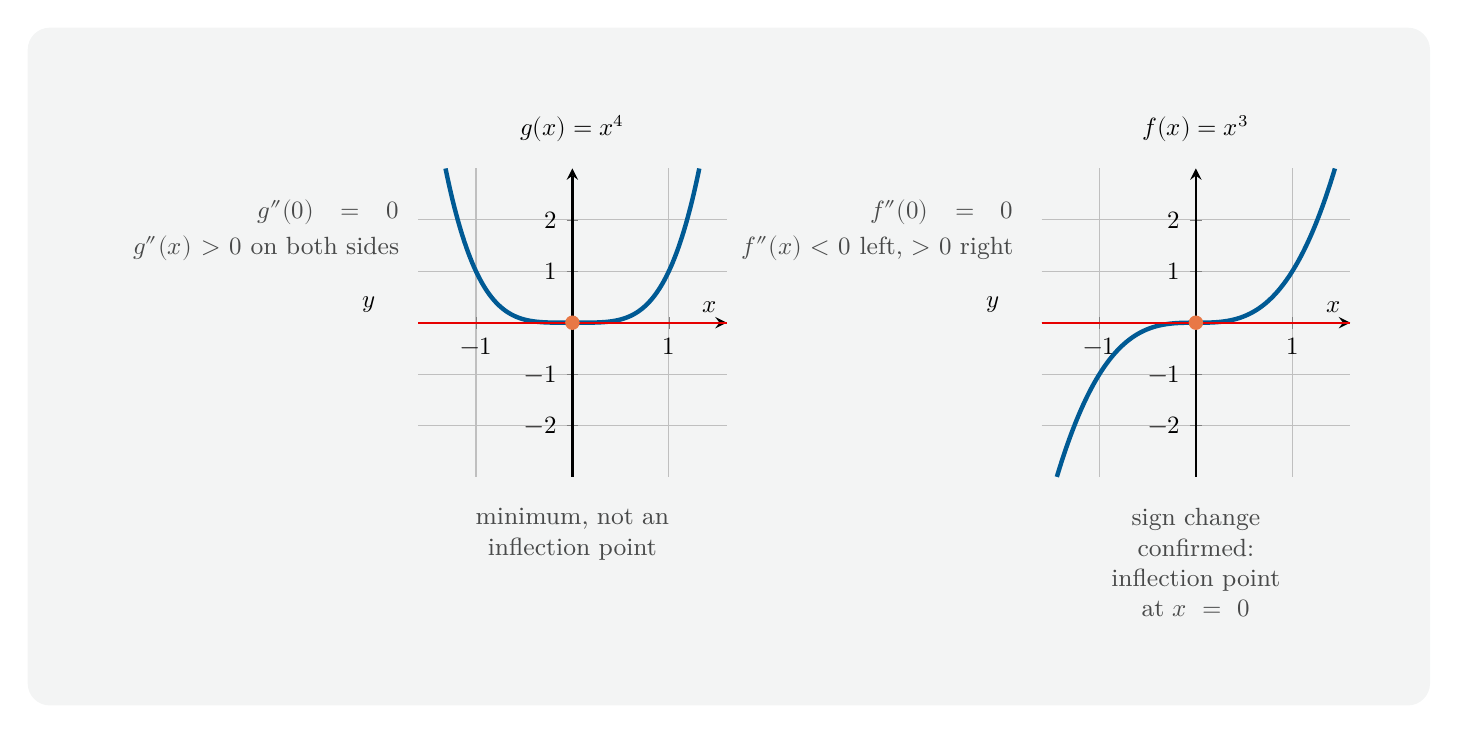
\begin{tikzpicture}[
  show background rectangle,
  background rectangle/.style={fill=my_lightgray, rounded corners=8pt},
  inner frame sep=1cm
]

\begin{groupplot}[
    group style={
      group size=2 by 1,
      horizontal sep=4cm,
    },
    width=5.5cm,
    height=5.5cm,
    axis lines=center,
    xmin=-1.6, xmax=1.6,
    ymin=-3, ymax=3,
    xtick={-1,0,1},
    ytick={-2,-1,0,1,2},
    grid=major,
    axis line style={thick},
    ticklabel style={font=\small},
    label style={font=\small},
    clip=false,
]

% -------- LEFT PANEL: g(x) = x^4 --------
\nextgroupplot[
    xlabel={$x$},
    ylabel={$y$},
    title={\small $g(x) = x^4$},
    ylabel style={
      at={(axis description cs:-0.16,0.5)},
      anchor=south
    },
]

% graph of x^4, clipped to ymax=3 at x = 3^(1/4) ≈ 1.316
\addplot[
    draw=my_darkblue,
    ultra thick,
    samples=200,
    domain=-1.316:1.316
]
{x^4};

% tangent at x=0: y = 0
\addplot[
    draw=my_red,
    thick,
    domain=-1.6:1.6,
    samples=2
]
{0};

% point at origin
\addplot[
    only marks,
    mark=*,
    mark size=2.4pt,
    draw=my_orange,
    fill=my_orange
]
coordinates {(0,0)};

% left annotation: anchor=east, placed just outside the left axis boundary
\node[
    anchor=east,
    font=\small,
    my_darkgray,
    text width=3.6cm,
    align=right
]
at (axis description cs:-0.03, 0.8)
{$g''(0)=0$\\[2pt]$g''(x)>0$ on both sides};

% bottom annotation: anchor=north, placed just below the axis
\node[
    anchor=north,
    font=\small,
    my_darkgray,
    text width=3cm,
    align=center
]
at (axis description cs:0.5, -0.07)
{minimum, not an inflection point};

% -------- RIGHT PANEL: f(x) = x^3 --------
\nextgroupplot[
    xlabel={$x$},
    ylabel={$y$},
    title={\small $f(x) = x^3$},
    ylabel style={
      at={(axis description cs:-0.16,0.5)},
      anchor=south
    },
]

% graph of x^3, clipped to ymin=-3 / ymax=3 at x = 3^(1/3) ≈ 1.442
\addplot[
    draw=my_darkblue,
    ultra thick,
    samples=200,
    domain=-1.442:1.442
]
{x^3};

% tangent at x=0: y = 0
\addplot[
    draw=my_red,
    thick,
    domain=-1.6:1.6,
    samples=2
]
{0};

% point at origin
\addplot[
    only marks,
    mark=*,
    mark size=2.4pt,
    draw=my_orange,
    fill=my_orange
]
coordinates {(0,0)};

% left annotation: anchor=east, placed just outside the left axis boundary
\node[
    anchor=east,
    font=\small,
    my_darkgray,
    text width=3.6cm,
    align=right
]
at (axis description cs:-0.06, 0.8)
{$f''(0)=0$\\[2pt]$f''(x)<0$ left, $>0$ right};

% bottom annotation: anchor=north, placed just below the axis
\node[
    anchor=north,
    font=\small,
    my_darkgray,
    text width=3cm,
    align=center
]
at (axis description cs:0.5, -0.07)
{sign change confirmed:\\inflection point at $x=0$};

\end{groupplot}

\end{tikzpicture}

\end{document}